\documentclass{article}

%math package
\usepackage{amsmath}
\usepackage{amsthm}
\usepackage{amsfonts}
\usepackage{amssymb}
%document package
\usepackage[utf8]{vietnam}
\usepackage{titlesec}
\usepackage{listings}
\usepackage{graphicx}
\usepackage[document]{ragged2e}
\usepackage{caption}
\usepackage{soul}
\usepackage{float}
\usepackage{subfigure}
\usepackage{multirow}
\usepackage{longtable}


%setup environment
\setcounter{secnumdepth}{4}
\graphicspath{{images/}}
%
\captionsetup{belowskip=12pt,aboveskip=4pt}
\begin{document}
	
%--------------------------title page-------------------------------------
\thispagestyle{empty}
\begin{titlepage}
\begin{center}
	\textbf{\huge{Khai thác dữ liệu và ứng dụng}}\\
	\Large{BT01: Khai thác tập phổ biến \& Luật kết hợp}	
\end{center}	

\vfill
\begin{flushright}
	\begin{tabular}{l l l}
		GVLT: & \quad Thầy Lê Hoài Bắc\\
		GVTH: & \quad Thầy Nguyễn Tiến Huy\\
		Sinh viên: & \quad Nguyễn Phan Mạnh Hùng & 1312727\\
		& \quad La Ngọc Thùy An & 1312716\\
	\end{tabular}
\end{flushright}
\end{titlepage}
\pagebreak
%-------------------------Mục lục-----------------------------------------
\thispagestyle{empty}
\tableofcontents
\pagebreak 
%-------------------------Bài 1------------------------------------------- 
\pagenumbering{arabic}
\section{Bài 1: Apriori}\label{sec: prob1}
\subsection{Câu 1}
\subsubsection{Tập phổ biến}

\begin{longtable}{c | c | c | c}

	Kích thướng & ID & Tập phổ biến  & Support \\ \hline
	\multirow{7}{*}{1} & 1 & Bread & 4 \\
	&2& Peanuts & 4 \\
	&3& Milk & 6 \\
	&4& Fruit & 6 \\
	&5& Jam & 5 \\
	&6& Soda & 6 \\
	&7& Chips & 4 \\ 
	\hline
	\multirow{15}{*}{2}&8& Bread Milk& 3\\
	&9& Bread Jam& 4\\
	&10& Bread Soda& 3\\
	&11& Bread Chips& 3\\
	&12& Peanuts Milk& 3\\
	&13& Peanuts Fruit& 4\\
	&14& Milk Fruit& 5\\
	&15& Milk Jam& 4\\
	&16& Milk Soda& 5\\
	&17& Milk Chips & 3\\
	&18& Fruit Jam& 3\\
	&19&Fruit Soda& 4\\
	&20&Jam Soda& 4\\
	&21& Jam Chips& 3\\
	&22& Soda Chips& 4\\ 
	\hline
	\multirow{15}{*}{10}&23&Bread Milk Jam& 3\\
	&24&Bread Jam Soda& 3\\
	&25&Bread Jam Chips& 3\\
	&26&Bread Soda Chips& 3\\
	&27&Peanuts Milk Fruit& 3\\
	&28&Milk Fruit Jam& 3\\
	&29&Milk Fruit Soda& 4\\
	&30&Milk Jam Soda& 3\\
	&31&Milk Soda Chips& 3\\
	&32&Jam Soda Chips& 3\\
	\hline
	4&33&Bread Jam Soda Chips& 3\\
	
\end{longtable}
\subsubsection{Thiết lập tham số}
\begin{figure}[H]
	\centering
	\caption{Màn hình thiết lập tham số}
	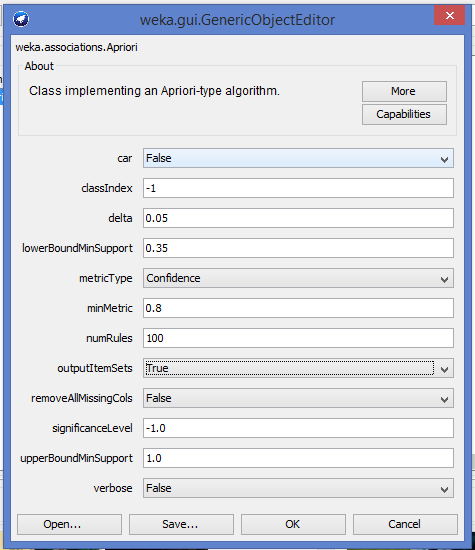
\includegraphics[scale = 0.5]{para}
\end{figure}

\subsection{Câu 2}
%\begin{tabular}
%\end{tabular}
\subsubsection{Luật kết hợp}
\begin{longtable}{c | c | c  c  c | c}
	
	
    Rule ID & Set ID & Rule &&& Confidence\\
    \hline
	1 & \multirow{2}{*}{8}&Bread 4 & $\to$ & Jam 4& 1\\ 
	2 & &Jam 5 & $\to$ & Bread 4& 0.8\\ \hline	
	3 & 13&Peanuts 4 & $\to$ & Fruit 4& 1\\ \hline	
	4 & 22&Chips 4 & $\to$ & Soda 4& 1\\ \hline	
	5 & \multirow{2}{*}{14}&Fruit 6 & $\to$ & Milk 5& 0.83\\
	6 & &Milk 6 & $\to$ & Fruit 5& 0.83\\ \hline	
	7 & \multirow{2}{*}{16}&Soda 6 & $\to$ & Milk 5& 0.83\\
	8 & &Milk 6 & $\to$ & Soda 5& 0.83\\ \hline	
	9 & 15&Jam 5 & $\to$ & Milk 4& 0.8\\ \hline	
	10& 20&Jam 5 & $\to$ & Soda 4& 0.8\\ \hline	
	11& 19&Fruit Soda 4 & $\to$ & Milk 4& 1\\ \hline	
	12& 23&Bread Milk 3 & $\to$ & Jam 3& 1\\ \hline	
	13& 24&Bread Soda 3 & $\to$ & Jam 3& 1\\ \hline	
	14& \multirow{2}{*}{25}&Jam Chips 3 & $\to$ & Bread 3& 1\\
	15& &Bread Chips 3 & $\to$ & Jam 3& 1\\	\hline
	16& \multirow{2}{*}{26}&Bread Chips 3 & $\to$ & Soda 3& 1\\
	17& &Bread Soda 3 & $\to$ & Chips 3& 1\\ \hline	
	18& 27&Peanuts Milk 3 & $\to$ & Fruit 3& 1\\ \hline
	19& 28&Fruit Jam 3 & $\to$ & Milk 3& 1\\ \hline	
	20& 31&Milk Chips 3 & $\to$ & Soda 3& 1\\ \hline	
	21& 32&Jam Chips 3 & $\to$ & Soda 3& 1\\ \hline	
	22& \multirow{2}{*}{29}&Milk Soda 5 & $\to$ & Fruit 4& 0.8\\
	23& &Milk Fruit 5 & $\to$ & Soda 4& 0.8\\ \hline	
	24& \multirow{7}{*}{33}&Jam Soda Chips 3 & $\to$ & Bread 3& 1\\
	25& &Bread Soda Chips 3 & $\to$ & Jam 3& 1\\
	26& &Bread Jam Chips 3 & $\to$ & Soda 3& 1\\
	27& &Bread Jam Soda 3 & $\to$ & Chips 3& 1\\
	28& &Jam Chips 3 & $\to$ & Bread Soda 3& 1\\
	29& &Bread Chips 3 & $\to$ & Jam Soda 3& 1\\
	30& &Bread Soda 3 & $\to$ & Jam Chips 3& 1\\
\end{longtable}
\subsubsection{Kết quả luật kết hợp}
\begin{figure}[H]
	\centering
	\caption{Kết quả luật kết hợp bằng Weka}
	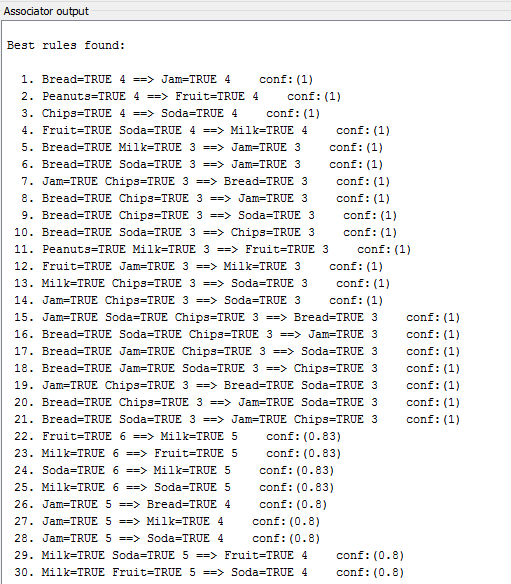
\includegraphics[scale = 0.7]{Rule}
\end{figure}
%-------------------------Bài 2------------------------------------------- 
\section{Bài 2: FP-Growth}\label{sec: prob2}
\subsection{Câu 1}
\begin{flushleft}
Bước 1: Duyệt cơ sở dữ liệu, chọn ra các item phổ biến và sắp xếp giảm dần. Ta được:\\
\begin{center}
\begin{tabular}{|c|c|c|c|c|c|c|}
	\hline Milk & Fruit & Soda & Jam & Chips & Peanuts & Bread \\ 
	\hline 6 & 6 & 6 & 5 & 4 & 4 & 4 \\ 
	\hline 
\end{tabular} 
\end{center}
Bước 2: Duyệt cơ sở dữ liệu lần hai. Với mỗi transaction, ta sắp xếp các item theo thứ tự độ phổ biến giảm dần trong bảng trên. Ta được:\\
\begin{center}
\begin{tabular}{c|c c c c c c }
	Tid & \multicolumn{6}{c}{Items}  \\ 
	\hline 1 & Milk & Fuit & Jam & Peanuts & Bread &  \\ 
	2 & Milk & Fruit & Soda & Jam & Chips & Bread \\ 
	3 & Soda & Jam & Chips & Bread &  &  \\ 
	4 & Milk & Fruit & Soda & Jam & Peanuts &  \\ 
	5 & Milk & Soda & Jam & Chips & Bread &  \\ 
	6 & Milk & Fruit & Soda & Chips &  &  \\ 
	7 & Milk & Fruit & Soda & Peanuts &  &  \\ 
	8 & Fruit & Peanuts &  &  &  &  \\ 
\end{tabular} 
\end{center}



Bước 3: Xây dựng cây FP-growth\\ 
\begin{center}
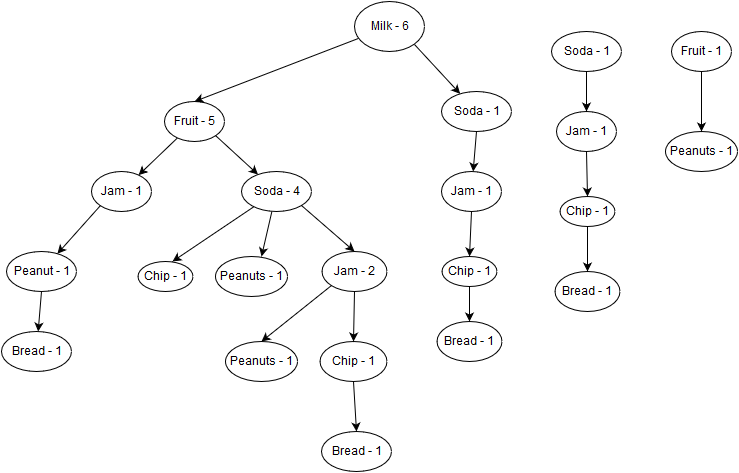
\includegraphics[scale = 0.5]{Tree.png}
\end{center}
Bước 4: Xây dựng các cơ sở dữ liệu điều kiện và sắp xếp theo thứ tự giảm dần của support.
\begin{table}[H]
	\centering
	\begin{minipage}[t]{\textwidth}
	\caption{CSDL điều kiện - Jam}
	\begin{tabular}{| c | c | c | c |}
		\hline
		Jam &&& \\ \hline
		&Milk - 1 & Fruit - 1 & \\ \hline
		&Milk - 2 & Soda - 2 & Fruit - 2  \\ \hline
		&Milk - 1 & Soda - 1 &  \\ \hline
		&Soda - 1 & & \\ \hline
	\end{tabular}
	\end{minipage}%
	\begin{minipage}[t]{\textwidth}
		\caption{CSDL điều kiện - Soda}
		\begin{tabular}{| c | c | c |}
			\hline
			Soda && \\ \hline
			&Milk - 4 & Fruit - 4  \\ \hline
			&Milk - 1 &  \\ \hline
		\end{tabular}
	\end{minipage}%
\end{table}
Ở đây ta được các tập phổ biến (ứng với mỗi điều kiện):\\
\begin{itemize}
	\item Bread
	\item Peanuts
	\item Chips
	\item Jam
	\item Soda
	\item Fruit
	\item Milk
\end{itemize}
Bước 5: Xây dựng các FP-trees tương ứng:
\begin{figure}[H]
	\centering
	\begin{minipage}[t]{0.5\textwidth}
		\centering
		\caption{Bread - FP tree}
		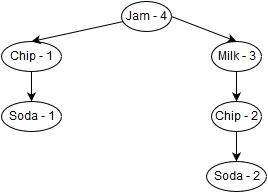
\includegraphics[scale = 0.5]{BreadTree}
	\end{minipage}%
	\begin{minipage}[t]{0.5\textwidth}
		\centering
		\caption{Peanuts - FP tree}
		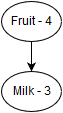
\includegraphics[scale = 0.5]{PeanutsTree}
	\end{minipage}
\end{figure}
\begin{figure}[H]
	\centering
	\begin{minipage}[t]{0.5\textwidth}
		\centering
		\caption{Chips - FP tree}
		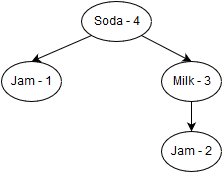
\includegraphics[scale = 0.5]{ChipsTree}
	\end{minipage}%
	\begin{minipage}[t]{0.5\textwidth}
		\centering
		\caption{Jam - FP tree}
		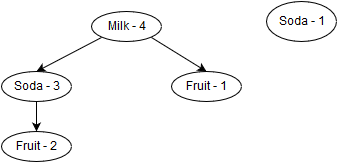
\includegraphics[scale = 0.5]{JamTree}
	\end{minipage}
\end{figure}
\begin{figure}[H]
	\centering
	\begin{minipage}[t]{0.5\textwidth}
		\centering
		\caption{Soda - FP tree}
		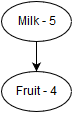
\includegraphics[scale = 0.5]{SodaTree}
	\end{minipage}%
	\begin{minipage}[t]{0.5\textwidth}
		\centering
		\caption{Fruit - FP tree}
		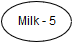
\includegraphics[scale = 0.5]{FruitTree}
	\end{minipage}
\end{figure}



Ta thấy các cây điều kiện Peanuts, Soda, và Fruit suy biến, nên ta tiến hành khai thác các tập phổ biến:
\begin{itemize}
	\item Peanuts Fruit
	\item Peanuts Milk
	\item Peanuts Fruit Milk
	\item Soda Fruit
	\item Soda Milk
	\item Soda Fruit Milk
	\item Fruit Milk
\end{itemize}
Sau đó ta lại tiếp tục đệ quy xây dựng các cơ sở dữ liệu điều kiện và cây FP cho tới khi các cây suy biến để khai thác tập phổ biến.\\
Cụ thể:\\
\begin{tabular}{|c|c|c|c|}
	\hline
	Điều kiện & Transactions & FP-tree & Tập phổ biến \\ 
	\hline
	Bread Soda & Chips - 1, Jam - 1 & (Chips - 3 $\to$ Jam - 3) & Bread Soda \\ 
	& Chips - 2, Jam - 2, \st{Milk} &  & Bread Soda Chips \\ 
	&  &  &  Bread Soda Jam\\
	&  &  &  Bread Soda Chips Jam\\ 
	\hline
	Bread Chips & Jam 1 & (Jam - 3) &Bread Chips\\
	& Jam - 2, \st{Milk} &  & Bread Chips Jam\\
	\hline
	Bread Milk & Jam - 3 & (Jam - 3)& Bread Milk\\
	&  &  &  Bread Milk Jam\\
	\hline
	Bread Jam & $\varnothing$ & $\varnothing$ &Bread Jam\\   
	\hline
	Chips Jam & Soda - 1 & (Soda - 3) & Chips Jam\\
	& Soda - 2, \st{Milk} &  & Chips Jam Soda\\
	\hline
	Chips Milk & Soda - 3 & (Soda - 3) & Chips Milk\\
	&  &  & Chips Milk Soda\\
	\hline
	Chips Soda & $\varnothing$ & $\varnothing$ & Chips Soda\\
	\hline
	Jam Fruit & Milk - 2, \st{Soda} & (Milk-3) & Jam Fruit\\
	& Milk - 1 &  & Jam Fruit Milk\\
	\hline
	Jam Soda & Milk - 3 & (Milk - 3) & Jam Soda \\
	&  &  & Jam Soda Milk\\
	\hline 
	Jam Milk & $\varnothing$ & $\varnothing$ & Jam Milk\\
	\hline
\end{tabular} 

\end{flushleft}
%-------------------------Bài 3------------------------------------------- 
\section{Bài 3: Các độ đo lý thú}\label{sec: prob3}
\subsection{Câu 1}
\begin{flushleft}
	\underline{Quy ước:}
	\begin{tabular}{l l}
		B, C: &  itemset\\
		$conf\left(B \to C\right)$: &  độ đo \textbf{confidence} của luật $B \to C$ \\
		$lift\left(B, C\right):$ &  độ đo \textbf{lift} của luật $B \to C$ và C $\to B$ (do có cách tính tương tự)\\
		$conv\left(B \to C\right):$ &  độ đo \textbf{conviction} của luật $B \to C$ \\ 
		$leve\left(B \to C\right):$ &  độ đo \textbf{leverage} của luật $B \to C$ \\
	\end{tabular}
\end{flushleft}
\subsubsection{Confidence}
\begin{equation}
	conf\left(B \to C \right) = \frac{sup \left( B \cup C \right)}{sup \left( B\right)}
\end{equation}
\subsubsection{Lift}
\begin{equation}
	lift\left( B,C \right) = \frac{conf\left( B \to C \right)}{sup \left( C \right)} = \frac{sup \left(B \cup C \right)}{sup \left( B\right) \times sup \left( C \right)}
\end{equation}
\subsubsection{Conviction}
\begin{equation}
	conv\left( B \to C \right) = \frac{1 - sup \left( C \right)}{1 - conf \left( B \to C \right)}
\end{equation}
\subsubsection{Leverage}
\begin{equation}
	leve(A \to C) = sup \left(B \cup C \right) - sup\left(B\right) \times sup\left(C\right)
\end{equation}

\subsection{Câu 2}

\begin{longtable}{c | c c c c}
	Rule Id & Confidence & Lift & Leverage & Conviction\\ \hline 
	1 & 1.00 & 1.60 & 0.19 & 0.00 \\ 
	2 & 0.80 & 1.60 & 0.19 & 0.00 \\ 
	3 & 1.00 & 1.33 & 0.13 & 0.00 \\ 
	4 & 1.00 & 1.33 & 0.13 & 0.00 \\ 
	5 & 0.83 & 1.11 & 0.06 & 0.00 \\ 
	6 & 0.83 & 1.11 & 0.06 & 0.00 \\ 
	7 & 0.83 & 1.11 & 0.06 & 0.00 \\ 
	8 & 0.83 & 1.11 & 0.06 & 0.00 \\ 
	9 & 0.80 & 1.07 & 0.03 & 0.00 \\ 
	10 & 0.80 & 1.07 & 0.03 & 0.00 \\ 
	11 & 1.00 & 1.33 & 0.13 & 0.00 \\ 
	12 & 1.00 & 1.60 & 0.14 & 0.00 \\ 
	13 & 1.00 & 1.60 & 0.14 & 0.00 \\ 
	14 & 1.00 & 2.00 & 0.19 & 0.00 \\ 
\end{longtable}%
\begin{longtable}{c | c c c c}
	15 & 1.00 & 1.60 & 0.14 & 0.00 \\ 
	16 & 1.00 & 1.33 & 0.09 & 0.00 \\ 
	17 & 1.00 & 2.00 & 0.19 & 0.00 \\ 
	18 & 1.00 & 1.33 & 0.09 & 0.00 \\ 
	19 & 1.00 & 1.33 & 0.09 & 0.00 \\ 
	20 & 1.00 & 1.33 & 0.09 & 0.00 \\ 
	21 & 1.00 & 1.33 & 0.09 & 0.00 \\ 
	22 & 0.80 & 1.07 & 0.03 & 0.00 \\ 
	23 & 0.80 & 1.07 & 0.03 & 0.00 \\ 
	24 & 1.00 & 2.00 & 0.19 & 0.00 \\ 
	25 & 1.00 & 1.60 & 0.14 & 0.00 \\ 
	26 & 1.00 & 1.33 & 0.09 & 0.00 \\ 
	27 & 1.00 & 2.00 & 0.19 & 0.00 \\ 
	28 & 1.00 & 2.67 & 0.23 & 0.00 \\ 
	29 & 1.00 & 2.00 & 0.19 & 0.00 \\ 
	30 & 1.00 & 2.67 & 0.23 & 0.00 \\ 
\end{longtable}

\subsection{Câu 3}
\begin{figure}[H]
	\centering
	\caption{Giá trị Confidence, Lift, Leverage, Conviction tính bằng Weka}
	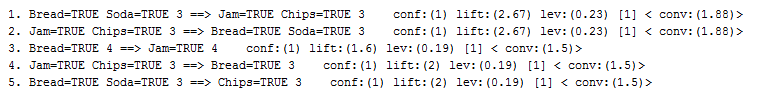
\includegraphics[scale = 0.8]{Measure}
\end{figure}
\end{document}